\section{Co-Regular of Priority Queues}
\label{sec:co-regular of priority queues}

A rule $R$ of priority queue is co-regular, if checking linearizability with respect to $\textit{MS}(R)$ of a data-independent implementation $\mathcal{I}$ can be reduced to checking the emptiness of intersection between $\mathcal{I}$ and a set of witness automata. In this section, we propose the definition of witness automata and co-regular. Then we prove that all five rules of priority queues are co-regular, and roughly introduce the proof idea. With the help of step-by-step linearizability and co-regular, we finally reduce the linearizability problem of $\textit{PQueue}$ into emptiness problem of intersection with automata.



\subsection{Definition of Co-Regular}
\label{subsec:definition of co-regular}

A witness automaton is a finite automaton with alphabet $\{ \textit{cal}(\textit{put},d,\textit{pre}), \textit{ret}(\textit{put}d),$ $\textit{cal}(\textit{rm},d),\textit{ret}(\textit{rm},d) \vert d \in \mathbb{D},\textit{red} \in \textit{preWA} \}$. Here $\textit{preWA}$ is the set of predicate of priorities, and it contains

\begin{itemize}
\setlength{\itemsep}{0.5pt}
\item[-] A predicate variable $p$, which accepts some specific priority,

\item[-] A predicate $\textit{les}_p$, which accepts all the priorities that are less than the value of $p$,

\item[-] A predicate $\textit{anyPri}$, which accepts any priority.
\end{itemize}

Given a execution $e = \alpha_1 \cdots \alpha_k$ of priority queue and a witness automaton $\mathcal{A}$, we say that $e$ is accepted by $\mathcal{A}$, if

\begin{itemize}
\setlength{\itemsep}{0.5pt}
\item[-] There exist transitions $q_0 \xrightarrow{\beta_1} q_1 \ldots \xrightarrow{\beta_k} q_k$ of $\mathcal{A}$, such that $q_0$ is one of initial state of $\mathcal{A}$, and $q_k$ is one of accept state of $\mathcal{A}$. Let $d_p \in \mathbb{D}$.

\item[-] For each $i$, if $\alpha_i = \textit{cal}(\textit{put},a,q)$, then either (1) $\beta_i = \textit{cal}(\textit{put},a,p)$ and $q = d_p$, or (2) $\beta_i = \textit{cal}(\textit{put},a,\textit{les}_p)$ and $q < d_p$, or (3) $beta_i = \textit{cal}(\textit{put},a,\textit{anyPri})$.

\item[-] For each $i$, if $\alpha_i = \textit{ret}(\textit{put},a)$, or $\alpha_i = \textit{cal}(\textit{rm},a)$, or $\alpha_i = \textit{ret}(\textit{rm},a)$, then $\beta_i = \alpha_i$.
\end{itemize}

Note that witness automata does not read operations, since the domains of operations is infinite.

Let us introduce the notion of co-regular:

%\vspace{-6pt}
\begin{definition}\label{def:co-regular of rules of priority queues}
A rule $R$ of priority queue is co-regular, if there are a finite set $\textit{Auts}_{R}$ of witness automata such that, for each data-independence implementation $\mathcal{I}$, we have that

$$ \textit{Auts}_{R} \cap \mathcal{I} = \emptyset \Leftrightarrow \exists e \in \mathcal{I}_{\neq},e' \in \textit{proj}(e), last(e')=R \wedge e \ does \ not \ linearizable \ w.r.t. \ \textit{MS}(R)$$

We say that $\textit{PQueue}$ is regular, if each of its rule is co-regular.
\end{definition}

Before we go to investigate co-regular of each rules, we use the results in \cite{Bouajjani:2015} to simplify our work. \cite{Bouajjani:2015} states that checking linearizability w.r.t queue can be reduced into checking emptiness of intersection between $\mathcal{I}$ and a set of automata. Given a data-differentiated execution $e$, let $e \vert_{i}$ be an execution generated from $e$ by erasing call and return actions of items that does not use priority $i$. We call a priority queue execution with only one priority a single-priority execution. Let $\textit{transToQueue}(e)$ be an execution generated from $e$ by transforming $\textit{put}$ and $\textit{rm}$ into $\textit{enq}$ and $\textit{deq}$, respectively, and then discarding priorities. We can see that for each $e \in \textit{PQueue}$ and each priority $i$, $\textit{transToQueue}(e \vert_{i})$ satisfy FIFO (first in first out) property.

Given an execution of queue, we say that it is differentiated \cite{Wolper:1986}, if each item is enqueued at most once. \cite{Bouajjani:2015} states that, given a differentiated queue execution $e$ without $\textit{deq}(\textit{empty})$, $e$ is not linearizable with respect to queue, if one of the following cases holds for some $a,b$: (1) $\textit{deq}(b) <_{hb} \textit{enq}(b)$, (2) there are are no $\textit{enq}(b)$ and least one $\textit{deq}(b)$, (3) there are are one $\textit{enq}(b)$ and more than one $\textit{deq}(b)$, and (4) $\textit{enq}(a) <_{\textit{hb}} \textit{enq}(b)$, and $\textit{deq}(b) <_{\textit{hb}} \textit{deq}(a)$, or $\textit{deq}(a)$ does not exists. For each such case, we can construct a witness automata for priority queue. For example, for the first case, we generate witness automata $\mathcal{A}_{\textit{SinPri}}^1$ in \figurename~\ref{fig:automata for FIFO-1}, here $c_1 = \textit{cal}(\textit{put},a,\textit{anyPri}), \textit{ret}(\textit{put},a), \textit{cal}(\textit{rm},a)$, $\textit{ret}(\textit{rm},a),\textit{cal}(\textit{rm},b)$, $c_2 = c_1 + \textit{ret}(\textit{rm},b)$, $c_3 = c_2 + \textit{ret}(\textit{put},b)$.


\begin{figure}[htbp]
  \centering
  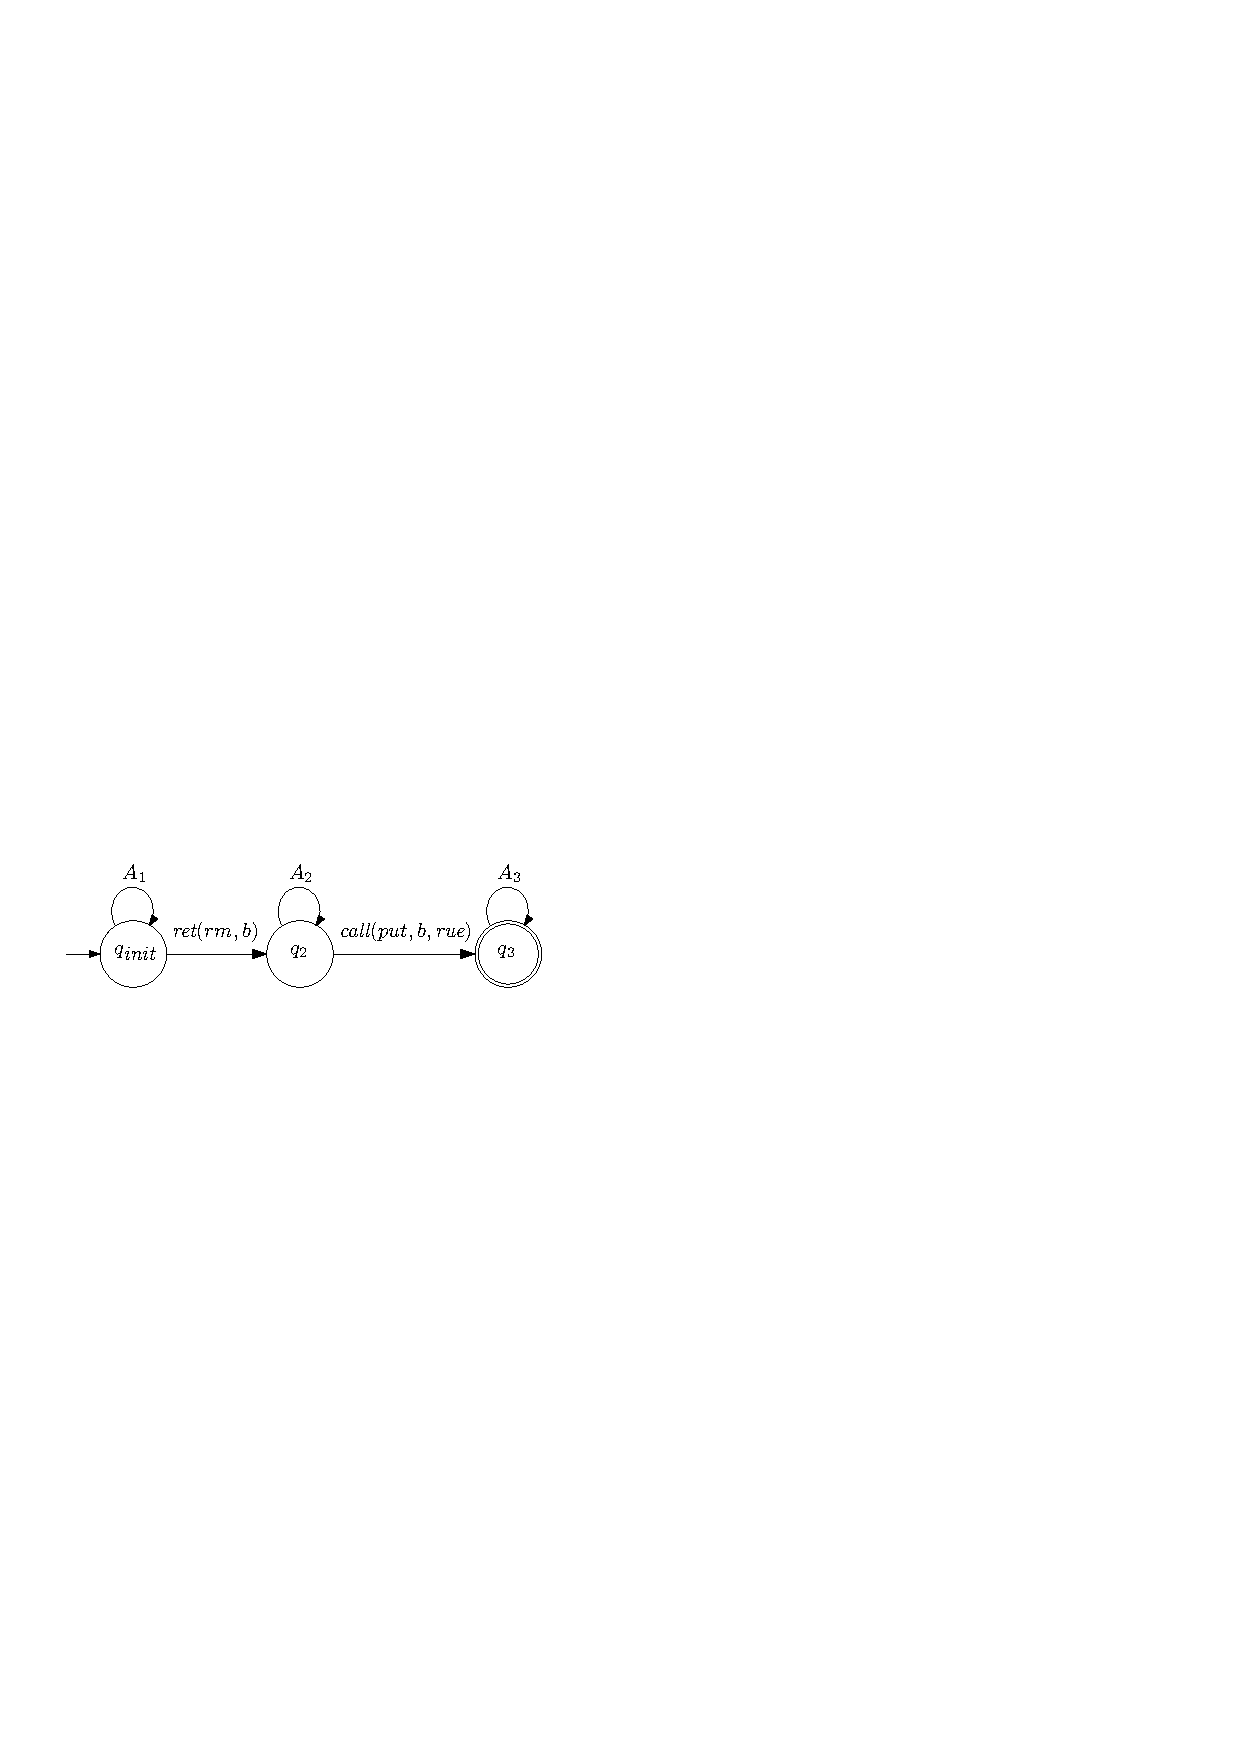
\includegraphics[width=0.6 \textwidth]{figures/PIC_AUTO_FIFO_1.pdf}
%\vspace{-10pt}
  \caption{Automaton $\mathcal{A}_{\textit{SinPri}}^1$}
  \label{fig:automata for FIFO-1}
\end{figure}

In Appendix \ref{sec:appendix proof and definition in section definition of co-regular}, we construct a set $\textit{Auts}_{\textit{sinPri}}$ of witness automata ($\mathcal{A}_{\textit{SinPri}}^1$ is in it), and shows that they are enough to ensure that for each of its data-differentiated executions, each of its single-priority projection that has no $\textit{rm}(\textit{empty})$ to have ``FIFO'' property, as shown by the following lemma.

\begin{restatable}{lemma}{AutoForPQwithSignlePri}
\label{lemma:automata for priority queue with single priority}

Given a data-independent implementations $\mathcal{I}$ of priority queue, $\mathcal{I} \cap \textit{Auts}_{\textit{sinPri}} \neq \emptyset$, if and only if there exists $e \in \mathcal{I}_{\neq}$, $e' \in \textit{proj}(e)$, such that $e'$ is single-priority  without $\textit{rm}(\textit{empty})$, and $\textit{transToQueue}(e')$ does not linearizable to queue.
\end{restatable}

According to Lemma \ref{lemma:automata for priority queue with single priority}, from now on, it is safe to assume that, for each data-differentiated execution without $\textit{rm}(\textit{empty})$, any of its single-priority projection has ``FIFO'' property. For example, $\textit{rm}(a)$ never happens before $\textit{put}(a,\_)$ for each $a$. 